\documentclass[12pt]{beamer}
\usepackage{outlines}

\usetheme{lugatuic}

\graphicspath{ {./images/} }


\title{Intro to VIM}
\titlegraphic{
\includegraphics[width=25mm]{lug-logo-invert.png}}
\author{Luke Deany}
\institute{Linux Users Group @ UIC}
\site{lug.cs.uic.edu}
\github{lugatuic}
\date{Fall 2025}

\setbeamertemplate{navigation symbols}{}

\begin{document}

\maketitle

\section{Overview}

\begin{frame}{Overview}
\begin{enumerate}
    \item What is Vim?
        \begin{itemize}
            \item An overview of what vim is, and why you should know how to use it.
        \end{itemize}

    \item How can I use Vim?
        \begin{itemize}
            \item An overview of how you can install vim, or simply how to use setup Vim keybinds in an editor of your choice
        \end{itemize}

    \item Vim Basics
        \begin{itemize}
            \item An overview of the basic commands you will use in vim just to get around
        \end{itemize}

    \item Interactive Vim Tutorial
        \begin{itemize}
            \item Finally, we’ll get you set up on an interactive tutorial for vim
        \end{itemize}
\end{enumerate}    
\end{frame}

\section{What is Vim}
\begin{frame}{What is Vim?}
\begin{outline}
\1 Vim stands for Vi iMproved
\2 Vi is an old text editor, so Vim is an improved version of this old text editor
\1 It’s primary draw is the many keyboard shortcuts
\1 It’s installed on pretty much every Linux machine
\1 Extensibility through plugins

\end{outline}
\end{frame}

\subsection{Why use keybinds?}

\begin{frame}{Why use keybinds?}

    \begin{columns}
        \column{0.42\textwidth} \begin{outline}
            \1 Less strain on wrists
            \2 Do not have to switch back to mouse
            \1 Increase in speed
            \1 Uniform across editors
        \end{outline}

        \column{0.58\textwidth} 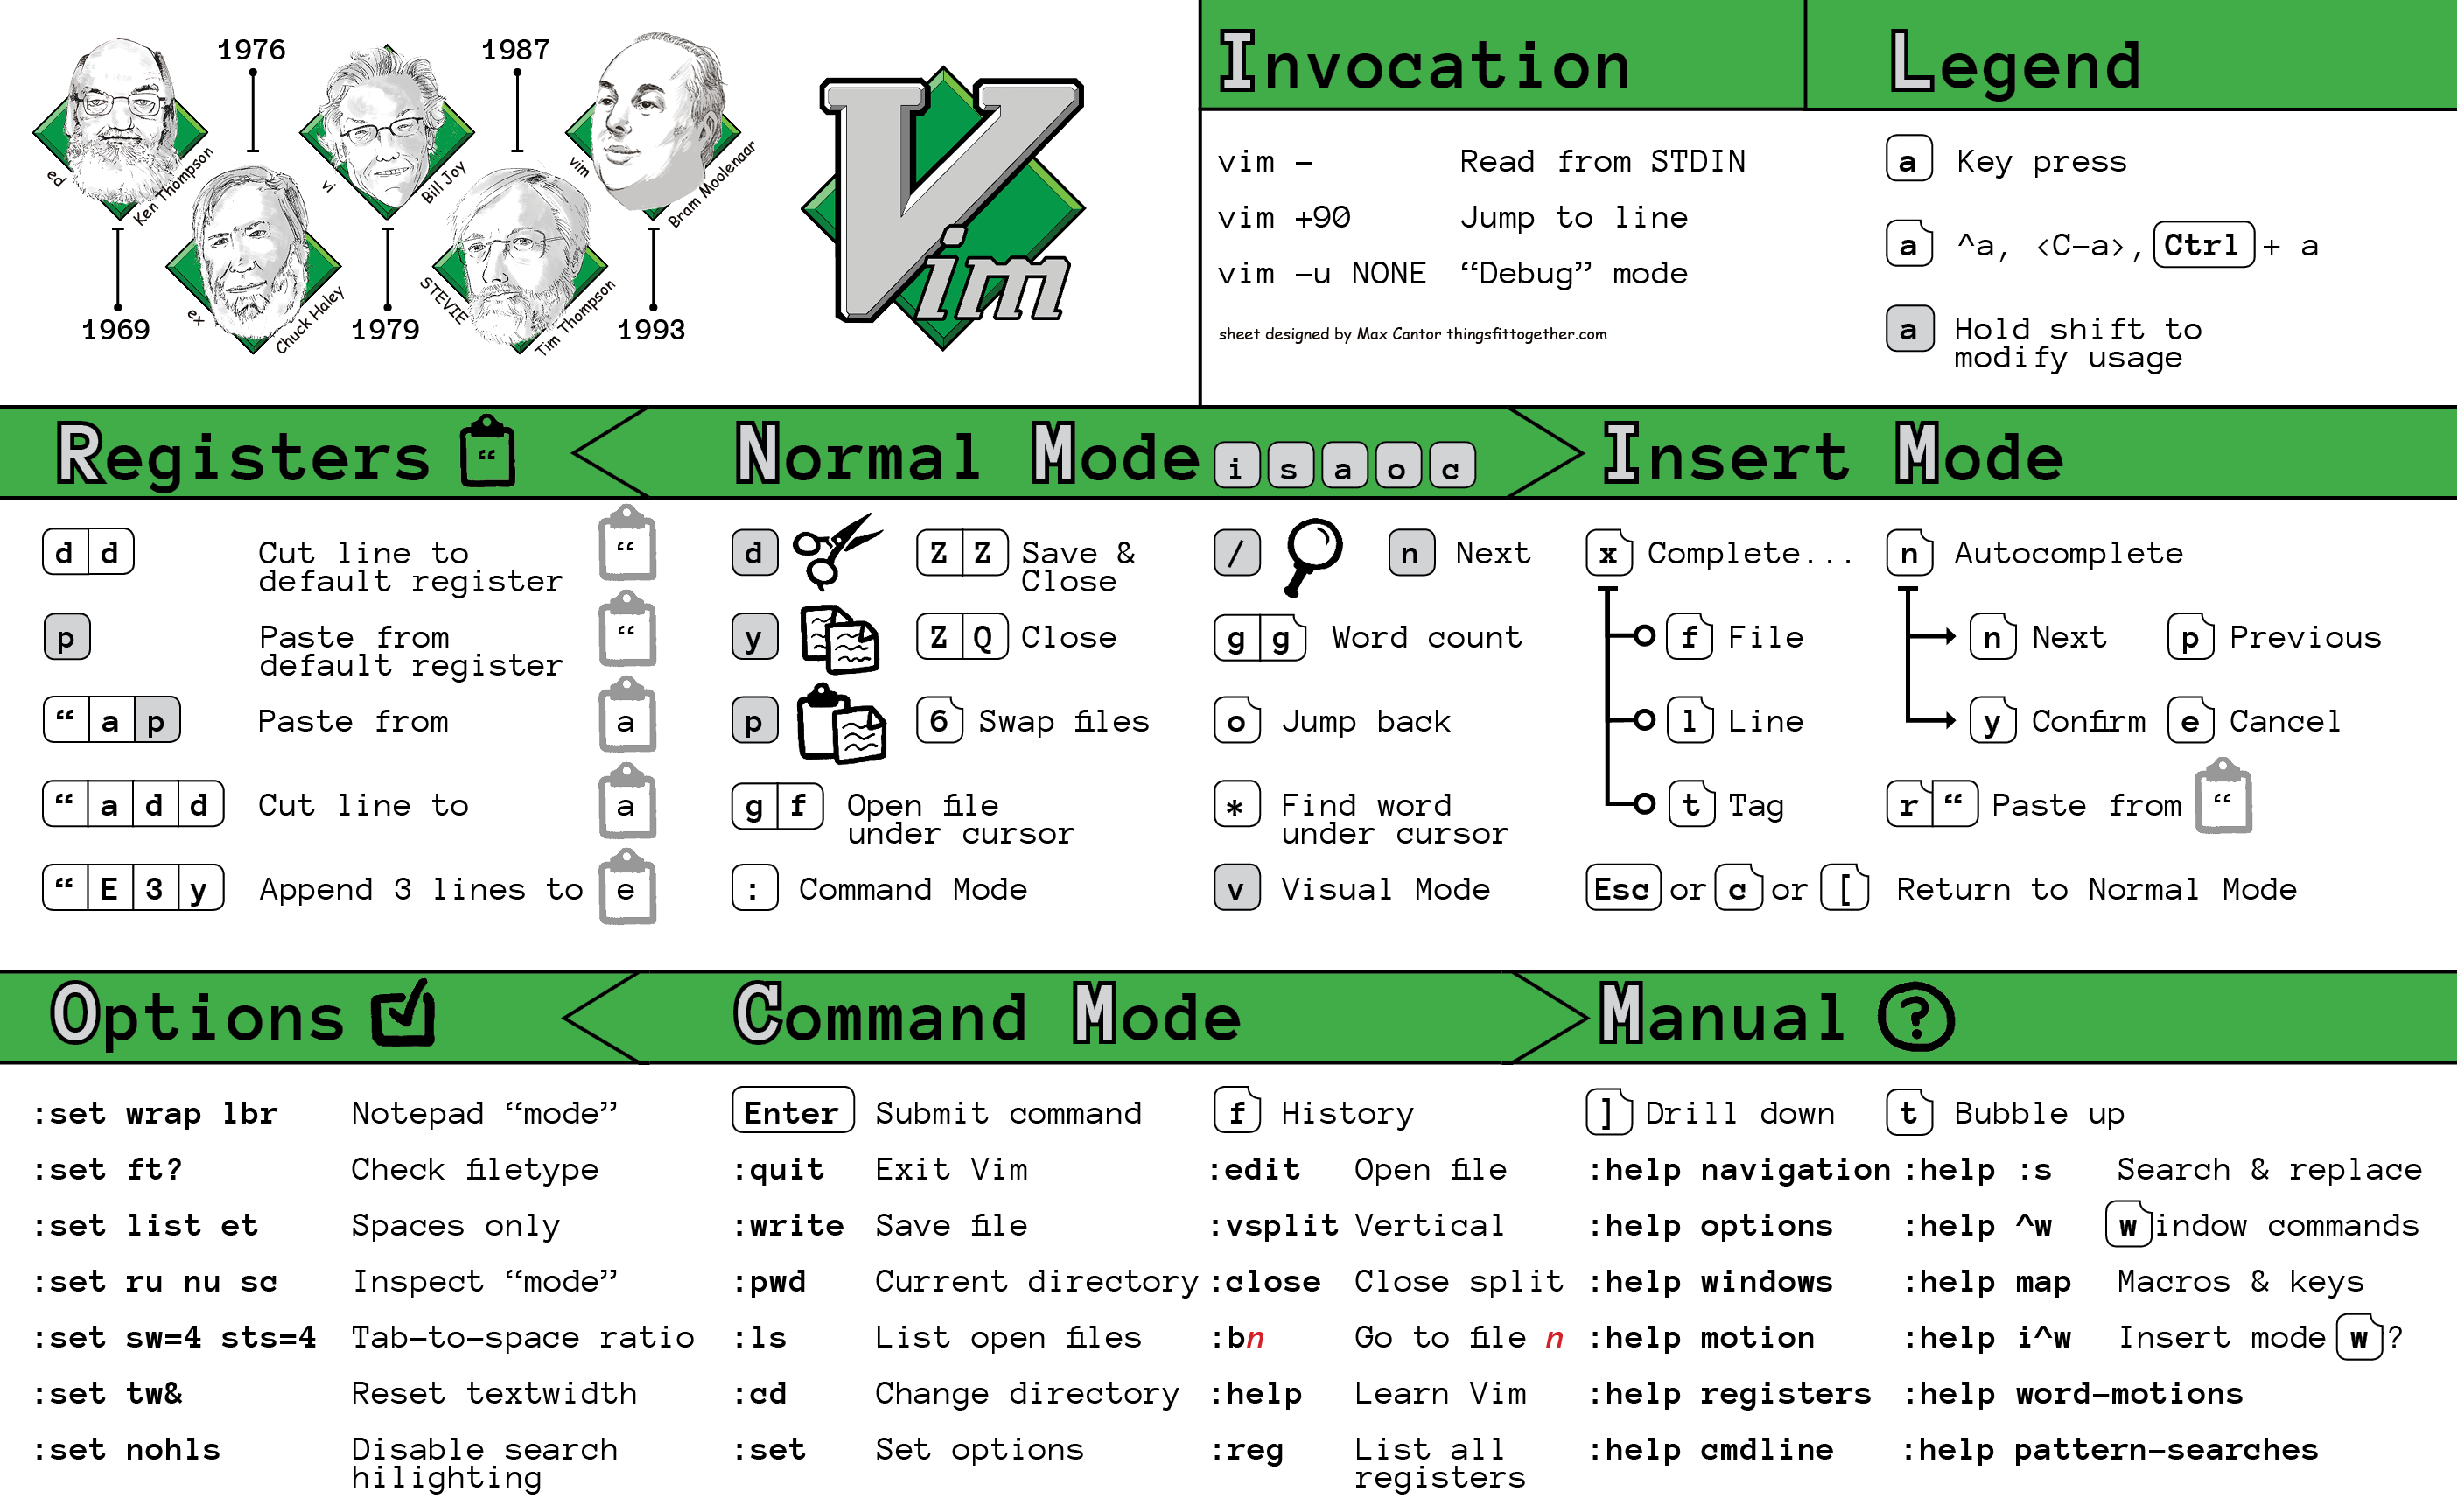
\includegraphics[width=\linewidth]{Vim-Cheatsheet-2-Final-Draft.png}\\
        {\tiny 
        https://thingsfittogether.com/product/vim-cheat-sheet-basics-print/}

    \end{columns}
    
\end{frame}

\section{How can I use Vim?}

\begin{frame}{How can I use Vim?}
    
    \begin{enumerate}
        {\scriptsize \item On Windows you can download Vim from their website, or using WSL (Windows Subsystem for Linux) will also have Vim installed}
{\scriptsize \item If you’re on a Linux machine, you already (most likely) have it installed, run “vim” in the terminal}
{\scriptsize \item MacOS has Vim installed by default, but it is a limited version, you can install the full version using homebrew}
    \end{enumerate}
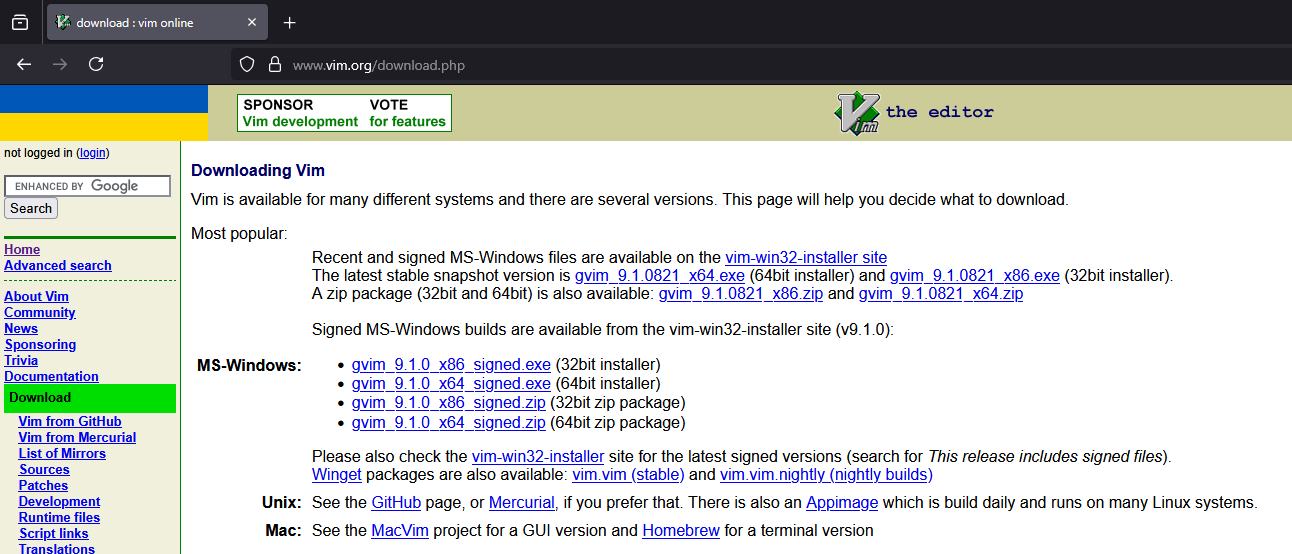
\includegraphics[width=\linewidth]{images/Vim-Download.PNG}
    
\end{frame}

\subsection{How can I use Vim keybinds?}

\begin{frame}{How can I use Vim?}
{\large How can I use Vim keybinds?}

\begin{columns}
    \column{0.7\textwidth} \begin{outline}
        \1 For pretty much every major editor, you have two options
        \2 Enable Vim mode if built-in
        \2 Install a Vim keybinds plugin
    \end{outline}
    \column{0.3\textwidth} 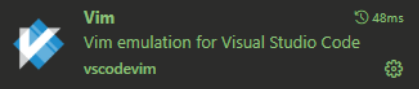
\includegraphics[width=\linewidth]{images/VimPlugin.PNG} 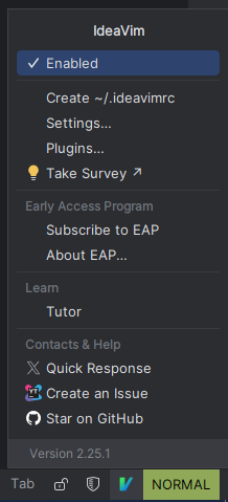
\includegraphics[width=\linewidth]{images/IdeaVim.PNG}
\end{columns}
    
\end{frame}

\section{Vim Basics}
\begin{frame}{Vim Basics}
TODO: Make intro page for vim basics
\end{frame}
\subsection{Modes}

\begin{frame}{Modes}
    {\large What are modes?}
    \begin{outline}
        \1 Modes are how you operate using vim, and each mode does different things. You can switch modes at pretty much any time.
        \2 This may be kind of confusing to think about at first, but you already are familiar with this concept if you use another development environment!
        \1 For instance, if you are writing code in visual studio code, and you then use your mouse to highlight text, you can think of it as "switching" into visual mode.
        \1 You can see what mode your in by checking the bottom left, but this may be changed by different vim configurations.
    \end{outline}
\end{frame}

\begin{frame}{Modes}
    {\large What modes are there?}
    \begin{outline}
    {
        \1 Normal Mode
        \2 {\scriptsize Vim “home base”, allows you to switch to different modes}
        \2 {\scriptsize Also used for things like rearranging text (copying and pasting)}
        \1Insert Mode
        \2 {\scriptsize The most common mode, in this mode any text you write will actually be written to the file}
        \1Visual Mode
        \2 {\scriptsize Allows you to select larger blocks of text visually, useful for copying and pasting, or deleting large sections}
        \1Command Mode
        \2 {\scriptsize Allows you to enter commands to Vim, which is used for things like saving, among plenty of other things}
        \1Replace Mode
        \2 {\scriptsize Like Insert Mode, but will directly write over text rather than adding new text}
        }
    \end{outline}
    
\end{frame}

\subsection{Buffers}
\begin{frame}{Buffers}
    \begin{outline}
        \1 Buffers are like the clipboard on your computer
\2 The buffer is separate from your clipboard
\2 Things you copy in vim will not copy to your clipboard, and vice versa
\1 You can have as many buffers as you want
\2 For this example we will stick to only 26, the characters in the English alphabet.
\1 Before inputting a command that uses buffers (you will see some in a second), you input double quote (") followed by the name of the buffer.
    \end{outline}
\end{frame}

\end{document}
